% Chapter Template

\chapter{Hardware Implementation of the FM-Index} % Main chapter title

\label{Chapter3} % Change X to a consecutive number; for referencing this chapter elsewhere, use \ref{ChapterX}			
The main scope of this thesis is to implement the aforementioned algorithm on a specific \textsl{FPGA} board, with all the reference data stored in a memory accessible via bus interface. This chapter will aim to describe a first implementation of this algorithm that could be duplicated on one board allowing them to run in parallel.

\section{Design}

Figures \ref{fig:seqschema} illustrate the hierarchy of the different blocks and element composing the \textsl{FM-Index}. \\

The details of the main FSM are described in Figure \ref{fig:seqschema}, the different blocks are described in Section 3.1.2. Note that there are two different data input sources : one that is used to receive actual sequences to map onto the reference, the other is used to configure the \textsl{Occ} array, used in the LastFirst Mapping.

\subsection{FM-Index}

\begin{figure}[H]   
    \centering
    \hspace*{-20mm}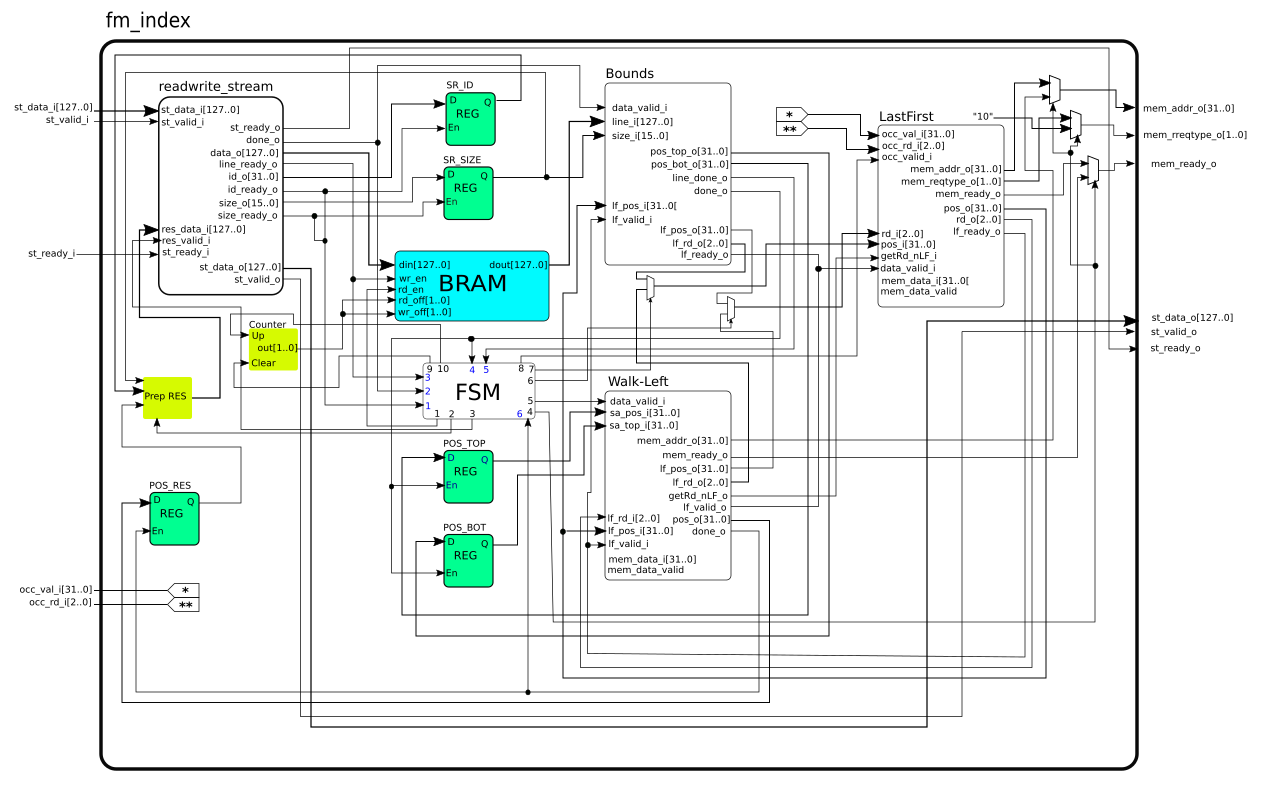
\includegraphics[scale = 0.45]{Figures/fmindex_top.png}
    \caption{Bloc Diagram of the FM-Index Top-Level}
    \label{fig:seqschema}
\end{figure}

This section illustrates the internal functioning of the \textsl{FM-Index} bloc, which is a hierarchical FSM, divided in 4 main steps as described below and illustrated in Figure \ref{fig:fm_fsm}.
\begin{description}
\item [Read Sequence -] This loop is used to consume data from the \textsl{PCI Express Interface} in order to load a short read to align in the reference text along with an ID value associated to it.
\item [Bounds] - This loop scans the input sequence $q$ and, at each iteration, queries the \textsl{HMC} memory to update $top$ and $bot$. Note that is corresponds to Algorithm \ref{alg:match}.
\item [Walk Left] - This loop corresponds to Algorithm \ref{alg:WL}. It is only reached when the precedent loop ends up with a valid range for $q$ in the suffix array, i.e. $q$ exists in the reference text. Then again, at each iteration, the HMC is queried to update the index.
\item [Send Result] - This last part of the FSM sends back the results, whether $q$ was found or not, back to the result FIFO in the \textsl{PCI Express Interface}. This result contains the position (special value if not found), along with the ID corresponding to the query, stored in the \textsl{Read Sequence} step.
\end{description}

\begin{minipage}[t]{0.45\textwidth}
\begin{figure}[H]
    \centering
    \hspace*{-25mm}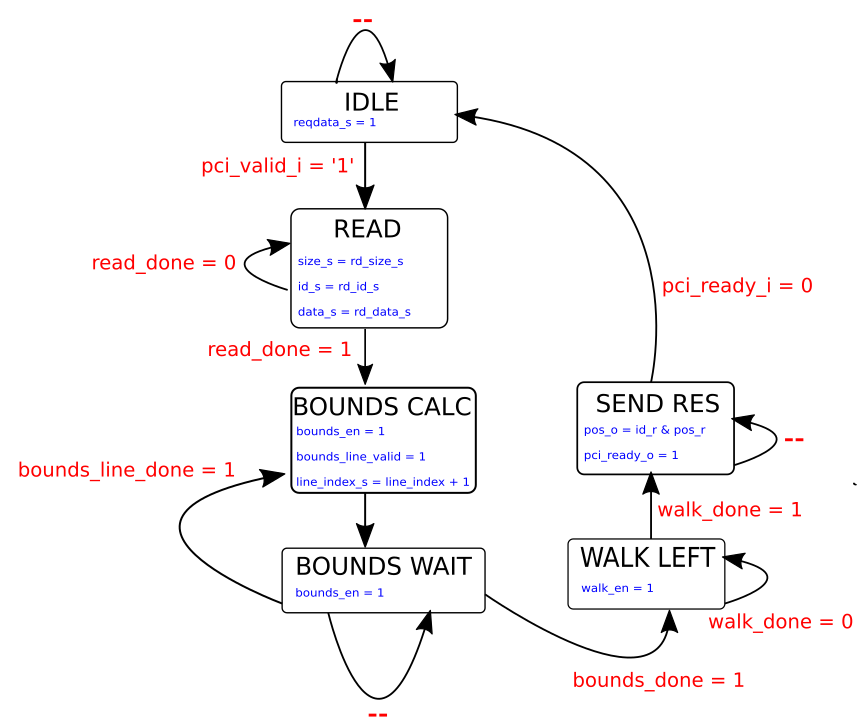
\includegraphics[scale = 0.37]{Figures/FM_FSM.png}
    \caption{FM-Index Main FSM}
    \label{fig:fm_fsm}
\end{figure}
\end{minipage}
\hfill
\begin{minipage}[t]{0.4\textwidth}
This finite state machine is rather simple. It waits until a new sequence to map becomes available then proceeds to wait for the ReadStream bloc to fetch, parse and store all data in the correct registers. \\

When all the data is ready to use, Bounds is automatically triggered and proceeds to iteratively scan the received sequence. Upon termination, Walk-Left starts automatically its execution. Between those two blocs, the FSM mainly has the role of an arbiter for the shared Last-First bloc and HMC Interface. The states

\end{minipage}


\subsection{Read\_Stream}

TODO

This block is responsible for reading the received data by the streaming bus. Those data start by the \textsl{short read} ID and size, followed by the actual sequence, already encoded and inverted. The first information are stored in registers and the short read itself is placed into a buffer : once a line is ready, the global FSM is notified, and the reading continues. \\
\vspace*{8mm}

\begin{minipage}[t]{0.45\textwidth}
\begin{figure}[H]
    \centering
    \hspace*{-20mm}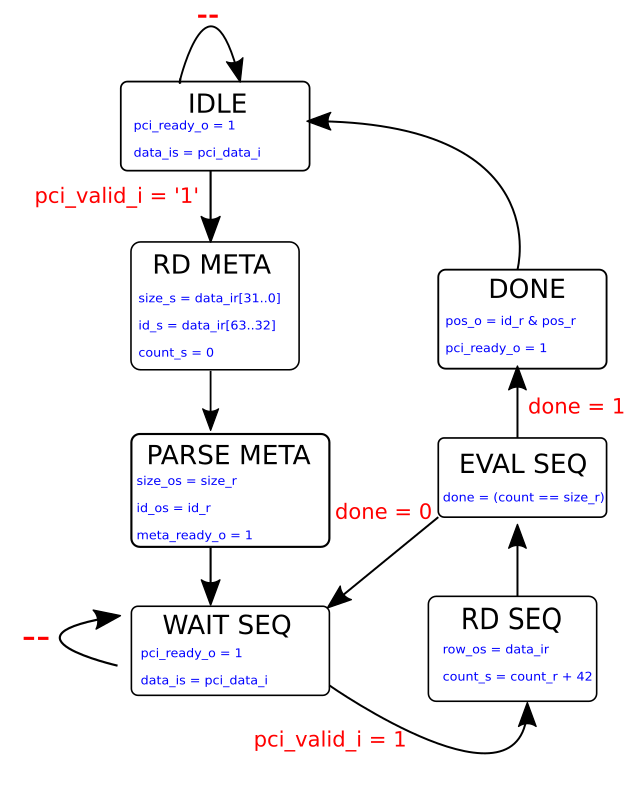
\includegraphics[scale = 0.4]{Figures/RDPCI_FSM.png}
    \caption{ReadStream Bloc FSM}
    \label{fig:bounds_fsm}
\end{figure}
\end{minipage}
\hfill
\begin{minipage}[t]{0.4\textwidth}
This sequential implementation of the Bounds algorithms is rather simple although not very time efficient. \\

At the INIT state, the first row of the short read to map is stored in an internal register and all the counters are reset to their initial values. After request and reception of the new values for both \textit{top} and \textit{bot}, an evaluation is done on those values (verifying that \textit{bot} > \textit{top}) and the current iteration number. \\
If the two positions are still correct and the whole row has not been read, it goes to the next symbol. If the current row is done but the short read is longer, the next row is requested.
\end{minipage}

\subsection{Bounds}


\begin{figure}[H]
    \centering
   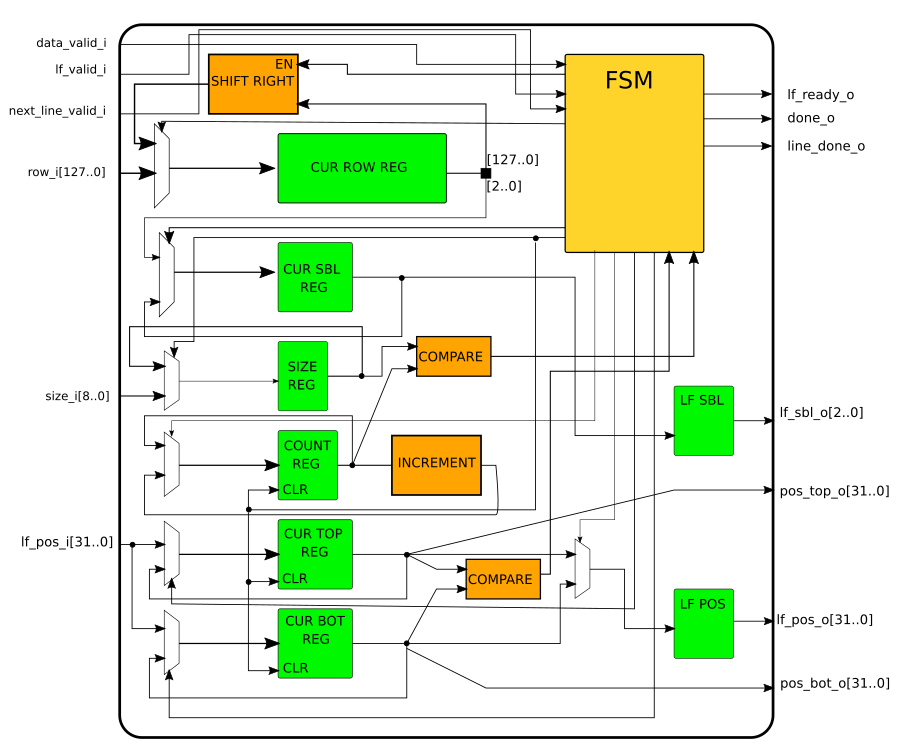
\includegraphics[scale = 0.4]{Figures/BOUNDS_DIAG.png}
    \caption{Bounds Bloc Diagram}
    \label{fig:bounds_diag}
\end{figure}



 This block reads this sequence from the buffer on line at a time, once all elements from it have been used, it notifies the upper level it is ready for the next one and continues until it has read \textrm{size} elements. For each read symbol iteration, the top and bottom position outputs are updated one after the other. After each update, both the number of read symbol and the new positions are evaluated and just like in Algorithm \ref{alg:match}, if at some point the interval $ [ top,bottom ] $ is empty, the loop is terminated the FSM goes back to waiting for a new sequence.

\begin{minipage}[t]{0.45\textwidth}
\begin{figure}[H]
    \centering
    \hspace*{-20mm}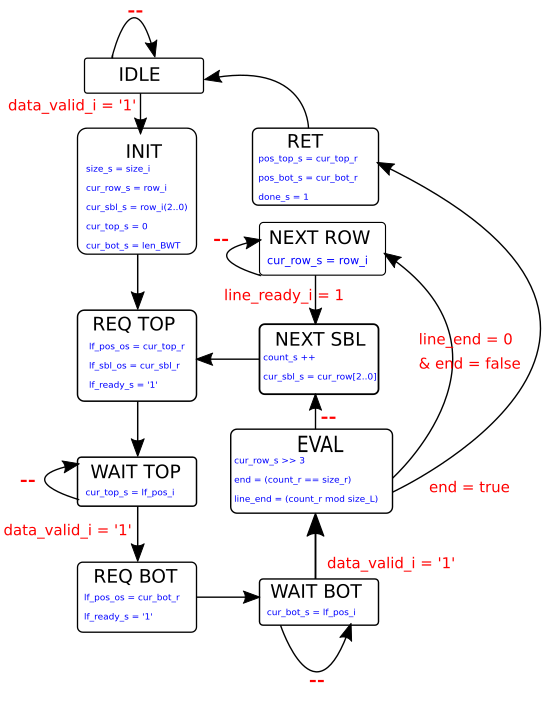
\includegraphics[scale = 0.5]{Figures/BOUNDS_FSM.png}
    \caption{Bounds Bloc FSM}
    \label{fig:bounds_fsm}
\end{figure}
\end{minipage}
\hfill
\begin{minipage}[t]{0.4\textwidth}
This sequential implementation of the Bounds algorithms is rather simple although not very time efficient. \\

At the INIT state, the first row of the short read to map is stored in an internal register and all the counters are reset to their initial values. After request and reception of the new values for both \textit{top} and \textit{bot}, an evaluation is done on those values (verifying that \textit{bot} > \textit{top}) and the current iteration number. \\
If the two positions are still correct and the whole row has not been read, it goes to the next symbol. If the current row is done but the short read is longer, the next row is requested.
\end{minipage}

\subsection{Walk-Left}

\begin{figure}[H]
    \centering
   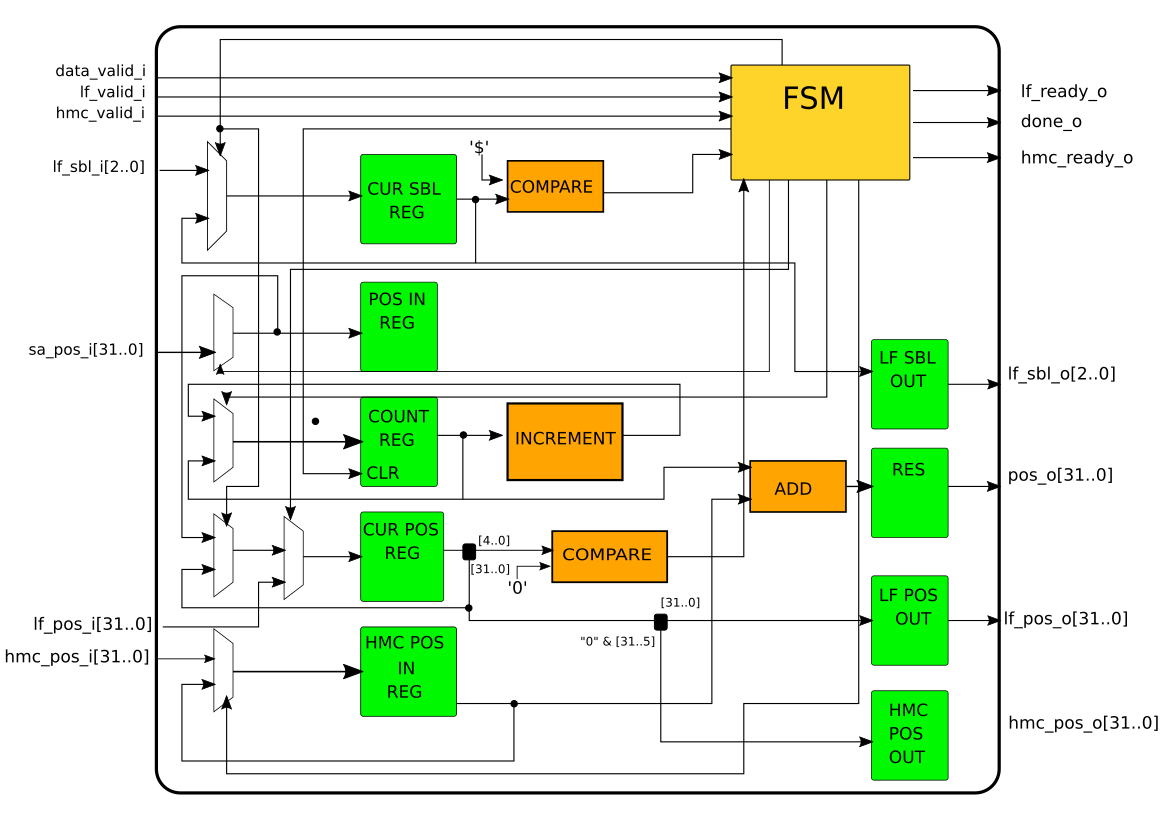
\includegraphics[scale = 0.4]{Figures/WL_DIAG.png}
    \caption{Walk-Left Bloc Diagram}
    \label{fig:bounds_diag}
\end{figure}

Upon termination of the \textsl{Bounds} algorithm, this block is notified that a new data is available. At the present time, only the \textsl{top} position is used. Hence, only one match - given there are at least one - is returned for each provided short read. As presented in Algorithm \ref{alg:WL}, this block first checks if there is a Suffix-Array index sample available for the provided position. If that's the case, it queries this value to the memory and returns it directly. If not, it fetches the BWT symbol corresponding to the current position and update this position using said symbol and said position for a LF-Mapping, and increments the number of step done so far. Then again, the new position is evaluated for a Suffix-Array index sample and so on and so forth until either the current position has such a sample, or the termination symbol \"\#\" is reached.
In the first case, the returned position is the number of step added to the index sample, in the latter, the number of steps is returned. \\

In both cases, the returned position corresponds to the short read position in the original (untransformed) text \textsl{T}.


\begin{minipage}[t]{0.45\textwidth}
\begin{figure}[H]
    \centering
    \hspace*{-25mm}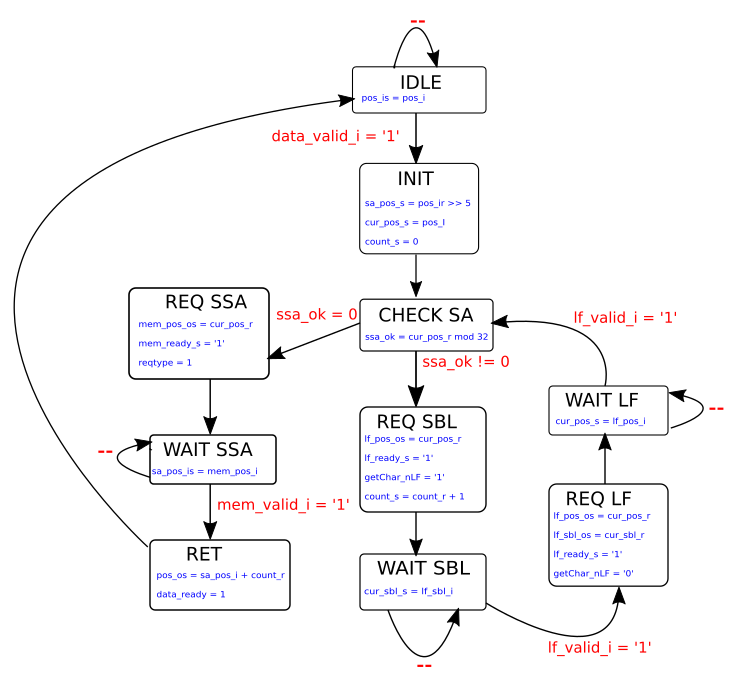
\includegraphics[scale = 0.45]{Figures/WL_FSM.png}
    \caption{Caption}
    \label{fig:wl_fsm}
\end{figure}
\end{minipage}
\hfill
\begin{minipage}[t]{0.3\textwidth}
TODO TODO TODO
\end{minipage}
\vspace*{8mm}


\subsection{Last-First}
\begin{figure}[H]
    \centering
   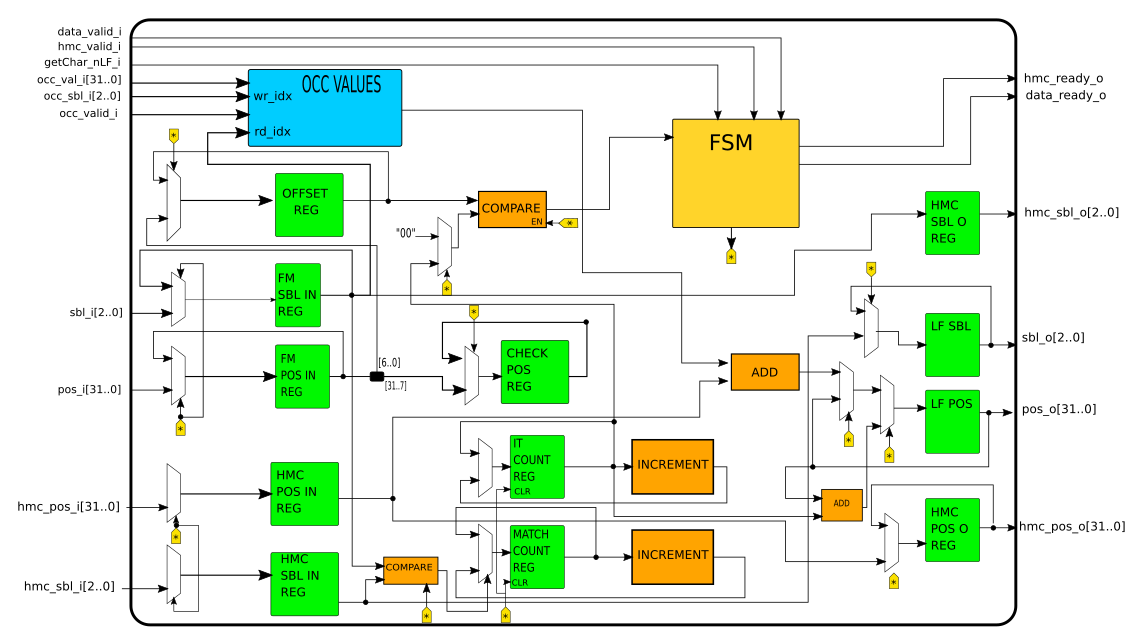
\includegraphics[scale = 0.4]{Figures/LF_DIAG.png}
    \caption{Last-Firt Mapping Bloc Diagram}
    \label{fig:bounds_diag}
\end{figure}

TODO

This block, used by both the \textsl{Bounds} and \textsl{Walk\_Left} blocks is the central processing unit of the FM-Index. This bloc aims to implement the mapping between the \textsl{BWT} symbols and their respective index in the conceptual suffix array first column (Equation \ref{eq:LF}. For each symbol of \textsl{T's} alphabet, its \textsl{Occ} value can be provided via a dedicated interface and placed into local registers. In order to determine the \textsl{Count} value of the provided inputs, it first queries the closest checkpoint value corresponding to the given symbol. It then iteratively queries \textsl{BWT} symbol from this position until it reaches the given position, incrementing a local count value each time the obtained symbol corresponds to the input.

Upon termination, the sum of all three values is returned. \\

Considering this methods of implementing \textsl{LF} requires querying symbols from the BWT, this block also provides this function to the rest of the system (only used by \textsl{Walk\_Left}, hence the input signal \textrm{getChar\_nLF\_i} that indicates which operation is demanded. To this end, an output signal \textrm{sbl\_o} is used to return the obtained symbol upon request.

\begin{figure}[H]
    \centering
\hspace*{-20mm}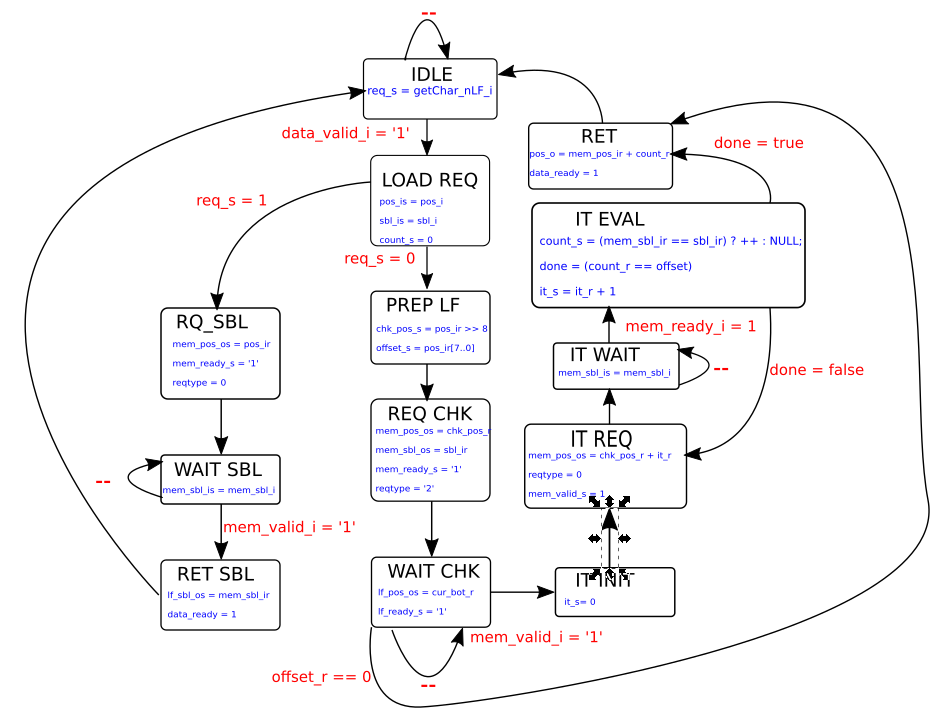
\includegraphics[scale = 0.5]{Figures/LF_FSM.png}
    \caption{Last-First Mapping FSM}
    \label{fig:lf_fsm}
\end{figure}
\vspace*{8mm}



\section{Test \& Validation}

In order to validate the behavior of the whole system while keeping good handle of its complexity, a testbench suite has been developped for each bloc composing the system, with a final one for the whole \textsl{FM-Index} bloc. \\

\subsection{References}
To simulate the memory, a reference dataset has been created using the previously introduced software. Using a reference text of length 1000, all the elements have been computed and place in reference files :

\begin{description}
\item [bwt\_pkg -] This file contains an array of all the BWT symbols in correct orders
\item [ssa\_pkg -] This file contains an array of all the sampled Suffix-Array indices
\item [chkX\_pkg -] Those files, one for each symbol A, C, G, T, and N contains an array of all the sampled checkpoints for each of those.
\item [lfX\_pkg -] Like the previous files, each one of those contains a lookup-table of Eq. \ref{eq:LF} for each possible entry.
\end{description}

\subsection{Global Structure}

\begin{figure}[H]
 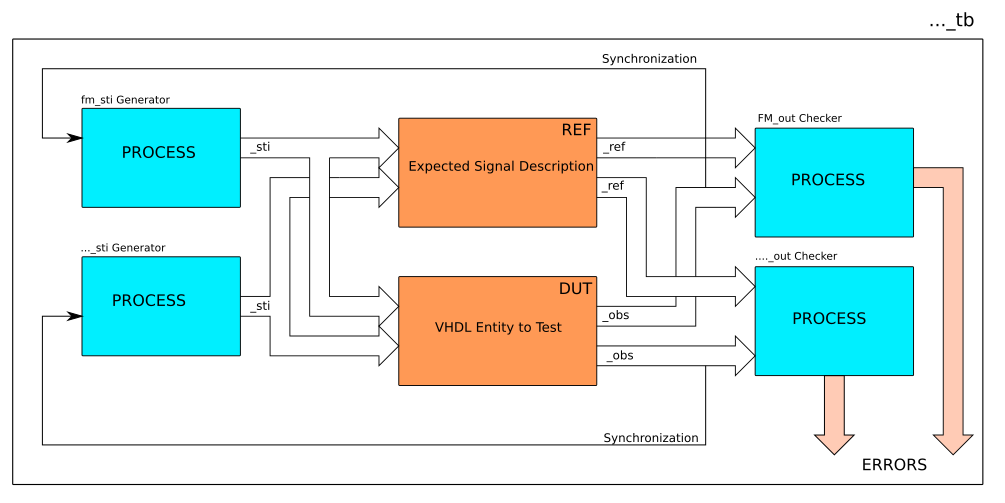
\includegraphics[scale = 0.4]{Figures/TB_struct.png}
    \caption{Global Structure of each Testbench}
    \label{fig:Tb_struct}
\end{figure}

Each testbench is defined according to the same structure, as depicted in Figure \ref{fig:Tb_struct}. For each DUT, a record is defined for each input sender and output receiver. For each input record, a process is defined to generate stimuli and for each output record, an equality operator is defined, allowing the \textrm{Verification} process to check the correctness of those output signals. \\
All DUT receive input from another internal block, referred as FM, which expects a final result. In order to get those results, most blocks need to interact with an external resource (such as a memory, a bus, etc.). Thus, those being independent in the computing process, it has been decided to completely separate those signals both in stimulation and verification. \\

Finally, every testbench includes two processes to generate a clock signal and an initial reset signal. The first is stopped upon the termination of the FM-stimuli. \\

The following paragraphs further detail those different input and output for each block and summarize the operations performed.


\subsection{Read PCI}
\vspace*{3mm}
\begin{center}
    \begin{tabular}{|c|c|}
\hline
  Input Src   &  Description \\
  \hline
   Stream  & Incoming data from the computer master (short reads) \\
   FM-Index & Result data to send back and data request \\
   \hline
\end{tabular}
\end{center}
\vspace*{5mm}

Upon availability of incoming data from the stream, the block should consume it as soon as the FM-Index is ready to process a new sequence. The other way, upon availability of a result from the FM-Index, it should send it out on the stream as soon a it becomes available.
\begin{center}
\begin{tabular}{|c|c|}
\hline
  Output Dest   &  Description \\
  \hline
   Stream  & Result Data (position, id) \\
   FM-Index & Data to process (id, size, sequence) \\
   \hline
\end{tabular}
\end{center}
\vspace*{5mm}
Data from received from the stream should be parsed correctly before being sent out to the FM-Index, meaning extracting the sequence's size and ID from the first packet and then fill the buffer line by line according to the previously received size. The other way around, it should push on the bus the final results provided by the FM-Index. \\


Following those properties, two cases are implemented in order to fully verify them :
\begin{itemize}
    \item [-] Simulate an incoming sequence from the stream and verify the FM-Index outputs
    \item [-] Simulate incoming results from the FM-Index and verify the stream outputs.
\end{itemize}


\subsection{Bounds}
\vspace*{3mm}
\begin{center}
    \begin{tabular}{|c|c|}
\hline
  Input Src   &  Description \\
  \hline
   FM-Index  & Validity flag, sequence row and size \\
   Last-First & Position result from made requests \\
   \hline
\end{tabular}
\end{center}
\vspace*{5mm}

When a new sequence becomes available, the DUT should immediately start to scann it, starting from the initial positions and, for each symbol, update those position using the Last-First Mapping algorithm (Eq. \ref{eq:LF}). Upon the reception of such a result, it should either go to the next symbol, request the next line if the current has been scanned, or terminate if all the sequence has been read, returning the final \textsl{top} and \textsl{bottom} positions. Note that the termination of the algorithm might be caused by obtaining an empty range, in which case the DUT should not keep scanning. \\
\begin{center}
\begin{tabular}{|c|c|}
\hline
  Output Dest   &  Description \\
  \hline
   FM-Index  & Validity flag, sequence row and size \\
   Last-First & Position result from made requests \\
   \hline
\end{tabular}
\end{center}
\vspace*{5mm}
For each symbol in the sequence, the correct queries should be made to Last-First, meaning the correct position and symbol. Finally, upon termination of the algorithm, the correct position should be returned.

Following those properties, two cases are implemented in order to fully verify them, using the LF references to generate Last-First stimuli :
\begin{itemize}
    \item [-] Simulate an incoming sequence present in the text and generate LF results upon request. Upon termination, verify the position outputs.
    \item [-]  Simulate an incoming sequence not present in the text and generate LF results upon request. Make sure of the early termination (less loop iteration than there are symbol in the sequence).
\end{itemize}

\subsection{Last-First}

\vspace*{3mm}
\begin{center}
    \begin{tabular}{|c|c|}
\hline
  Input Src   &  Description \\
  \hline
   FM-Index  & Position, symbol and operation type \\
   Memory & Position or BWT line \\
   \hline
\end{tabular}
\end{center}
\vspace*{5mm}

Upon a new request, the DUT should prepare the correct request to the memory. Upon reception of requested data from memory, it should use it to correctly continue its execution.

\begin{center}
\begin{tabular}{|c|c|}
\hline
  Output Dest   &  Description \\
  \hline
   FM-Index  & Position or BWT symbol \\
   Last-First & Position or symbol \\
   Memory & Position and request type \\
   \hline
\end{tabular}
\end{center}

Depending on the desired data, either a checkpoint position or a sample of the BWT, the correct outputs should be given to the memory interface. Upon termination of the algorithm, the correct value should be given to the FM-Index.

Following those properties, two cases are implemented in order to fully verify them, using the checkpoints and BWT references to generate memory stimuli :
\begin{itemize}
    \item [-] Simulate a position request and verify the sequence of request made to the memory in addition to the final results. 
    \item [-] Do the same simulatin a symbol request.
\end{itemize}
\subsection{Walk-Left}

\vspace*{3mm}
\begin{center}
    \begin{tabular}{|c|c|}
\hline
  Input Src   &  Description \\
  \hline
   FM-Index  & Position, symbol and operation type \\
   Last-First & Position and symbol \\
   Memory & Suffix-Array sample \\
   \hline
\end{tabular}
\end{center}
\vspace*{5mm}

Upon the availability of new data, the DUT should start immediatly to execute its algorithm. It should updates internal registers upon reception of Last-First (and potentially terminate) and terminate upon reception of memory data (retrieving a Suffix-Array sample leading to the final result).

\begin{center}
\begin{tabular}{|c|c|}
\hline
  Output Dest   &  Description \\
  \hline
    FM-Index  & Position of the short read in the text \\
   Last-First & Position, symbol and request type
   Memory & Position \\
   \hline
\end{tabular}
\end{center}

The DUT algorithm should be able to query symbols and positions from Last-First and a Suffix-Array from the memory. Upon termination, it should provide the correct value to the FM-Index interface.

Following those properties, several cases involving multiple positions are implemented, using the Suffiy-Array, the LFs and BWT references to generate memory stimuli. A loop is then done on a pre-defined array of test values.

\subsection{FMIndex}

\vspace*{3mm}
\begin{center}
    \begin{tabular}{|c|c|c|}
\hline
  Interfaces & Direction  &  Description \\
  \hline
   Stream & In  & Short reads sequence with ID and size \\
   Stream & Out & Position in text T \\
   \hline
\end{tabular}
\end{center}
\vspace*{5mm}

Upon the availability of new data on the input stream, the DUT and its component should start to process those data. A result must be reached and sent on the ouput stream.

Using the checkpoints, Suffix-Array and BWT references to generate memory stimuli, two case are implemented, one involving a input present in the text, the position of which is then verified. And another one involving an input not present in the text.

\section{Test Results}

As a result of those tests and simulation, several timing issues have been detected. Indeed, the use of register to store the data and signals as flags to notify other blocks of data availability led to several synchronization problems. 

\begin{figure}[H]
    \centering
    \hspace*{-10mm}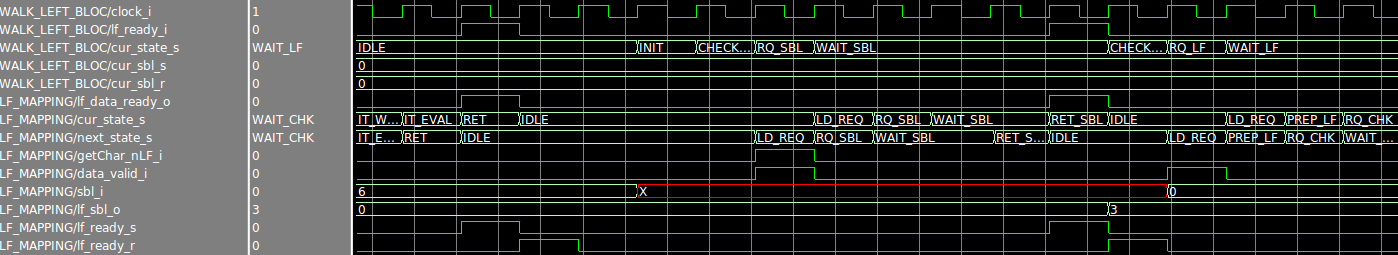
\includegraphics[scale = 0.5]{Figures/lf_timing_issue.png}
    \caption{TODO SANS X Example of Signal and Data Synchronization Issue}
    \label{fig:lf_timing}
\end{figure}

In this example, we see that the \textrm{data\_ready} output flag from the LF\_MAPPING bloc is issued using a signal, raised when it updates the output signal \textrm{sbl\_os}, the actual output value is only available on the next clock rising edge from the corresponding register. Hence, WALK-LEFT fetch the symbol value before it is updated, thus leading to a crash of the system. \\

Luckily, the solution to this kind of issue is rather simple : the output should be driven by the signal, which value is maintained using a register. Furthermore, considering it is a synchronous process that updates the flags, and thus the signals, the system remains fully synchronous.

[Mettre un autre truc qui allait pas]